\documentclass{extbook}[14pt]
\usepackage{multicol, enumerate, enumitem, hyperref, color, soul, setspace, parskip, fancyhdr, amssymb, amsthm, amsmath, latexsym, units, mathtools}
\everymath{\displaystyle}
\usepackage[headsep=0.5cm,headheight=0cm, left=1 in,right= 1 in,top= 1 in,bottom= 1 in]{geometry}
\usepackage{dashrule}  % Package to use the command below to create lines between items
\newcommand{\litem}[1]{\item #1

\rule{\textwidth}{0.4pt}}
\pagestyle{fancy}
\lhead{}
\chead{Answer Key for Progress Quiz 6 Version A}
\rhead{}
\lfoot{9689-6866}
\cfoot{}
\rfoot{Spring 2021}
\begin{document}
\textbf{This key should allow you to understand why you choose the option you did (beyond just getting a question right or wrong). \href{https://xronos.clas.ufl.edu/mac1105spring2020/courseDescriptionAndMisc/Exams/LearningFromResults}{More instructions on how to use this key can be found here}.}

\textbf{If you have a suggestion to make the keys better, \href{https://forms.gle/CZkbZmPbC9XALEE88}{please fill out the short survey here}.}

\textit{Note: This key is auto-generated and may contain issues and/or errors. The keys are reviewed after each exam to ensure grading is done accurately. If there are issues (like duplicate options), they are noted in the offline gradebook. The keys are a work-in-progress to give students as many resources to improve as possible.}

\rule{\textwidth}{0.4pt}

\begin{enumerate}\litem{
Construct the lowest-degree polynomial given the zeros below. Then, choose the intervals that contain the coefficients of the polynomial in the form $ax^3+bx^2+cx+d$.
\[ \frac{7}{3}, \frac{-5}{2}, \text{ and } \frac{-2}{3} \]The solution is \( 18x^{3} +15 x^{2} -103 x -70 \), which is option B.\begin{enumerate}[label=\Alph*.]
\item \( a \in [16, 21], b \in [-17, -12], c \in [-104, -99], \text{ and } d \in [68, 73] \)

$18x^{3} -15 x^{2} -103 x + 70$, which corresponds to multiplying out $(3x + 7)(2x -5)(3x -2)$.
\item \( a \in [16, 21], b \in [11, 20], c \in [-104, -99], \text{ and } d \in [-70, -68] \)

* $18x^{3} +15 x^{2} -103 x -70$, which is the correct option.
\item \( a \in [16, 21], b \in [8, 14], c \in [-111, -104], \text{ and } d \in [-70, -68] \)

$18x^{3} +9 x^{2} -107 x -70$, which corresponds to multiplying out $(3x + 7)(2x -5)(3x + 2)$.
\item \( a \in [16, 21], b \in [11, 20], c \in [-104, -99], \text{ and } d \in [68, 73] \)

$18x^{3} +15 x^{2} -103 x + 70$, which corresponds to multiplying everything correctly except the constant term.
\item \( a \in [16, 21], b \in [96, 104], c \in [162, 167], \text{ and } d \in [68, 73] \)

$18x^{3} +99 x^{2} +163 x + 70$, which corresponds to multiplying out $(3x + 7)(2x + 5)(3x + 2)$.
\end{enumerate}

\textbf{General Comment:} To construct the lowest-degree polynomial, you want to multiply out $(3x -7)(2x + 5)(3x + 2)$
}
\litem{
Describe the zero behavior of the zero $x = -2$ of the polynomial below.
\[ f(x) = 2(x + 2)^{8}(x - 2)^{11}(x + 9)^{3}(x - 9)^{6} \]The solution is the graph below, which is option B.
\begin{center}
    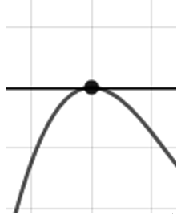
\includegraphics[width=0.3\textwidth]{../Figures/polyZeroBehaviorBA.png}
\end{center}\begin{enumerate}[label=\Alph*.]
\begin{multicols}{2}
\item 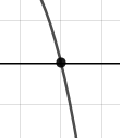
\includegraphics[width = 0.3\textwidth]{../Figures/polyZeroBehaviorAA.png}
\item 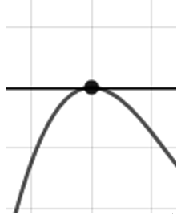
\includegraphics[width = 0.3\textwidth]{../Figures/polyZeroBehaviorBA.png}
\item 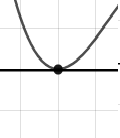
\includegraphics[width = 0.3\textwidth]{../Figures/polyZeroBehaviorCA.png}
\item 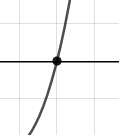
\includegraphics[width = 0.3\textwidth]{../Figures/polyZeroBehaviorDA.png}
\end{multicols}\item None of the above.\end{enumerate}
\textbf{General Comment:} You will need to sketch the entire graph, then zoom in on the zero the question asks about.
}
\litem{
Which of the following equations \textit{could} be of the graph presented below?

\begin{center}
    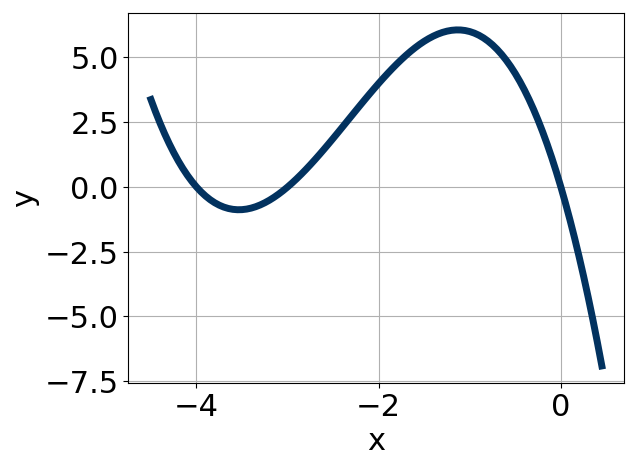
\includegraphics[width=0.5\textwidth]{../Figures/polyGraphToFunctionA.png}
\end{center}


The solution is \( 8x^{5} (x + 2)^{10} (x - 2)^{7} \), which is option D.\begin{enumerate}[label=\Alph*.]
\item \( 19x^{10} (x + 2)^{10} (x - 2)^{7} \)

The factor $x$ should have an odd power.
\item \( -4x^{7} (x + 2)^{8} (x - 2)^{5} \)

This corresponds to the leading coefficient being the opposite value than it should be.
\item \( -6x^{9} (x + 2)^{6} (x - 2)^{4} \)

The factor $(x - 2)$ should have an odd power and the leading coefficient should be the opposite sign.
\item \( 8x^{5} (x + 2)^{10} (x - 2)^{7} \)

* This is the correct option.
\item \( 5x^{4} (x + 2)^{9} (x - 2)^{7} \)

The factor $-2$ should have an even power and the factor $0$ should have an odd power.
\end{enumerate}

\textbf{General Comment:} General Comments: Draw the x-axis to determine which zeros are touching (and so have even multiplicity) or cross (and have odd multiplicity).
}
\litem{
Describe the zero behavior of the zero $x = 7$ of the polynomial below.
\[ f(x) = -2(x + 9)^{10}(x - 9)^{8}(x + 7)^{8}(x - 7)^{5} \]The solution is the graph below, which is option A.
\begin{center}
    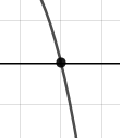
\includegraphics[width=0.3\textwidth]{../Figures/polyZeroBehaviorCopyAA.png}
\end{center}\begin{enumerate}[label=\Alph*.]
\begin{multicols}{2}
\item 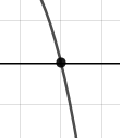
\includegraphics[width = 0.3\textwidth]{../Figures/polyZeroBehaviorCopyAA.png}
\item 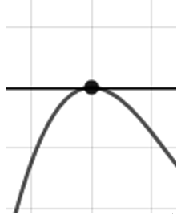
\includegraphics[width = 0.3\textwidth]{../Figures/polyZeroBehaviorCopyBA.png}
\item 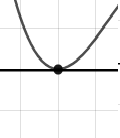
\includegraphics[width = 0.3\textwidth]{../Figures/polyZeroBehaviorCopyCA.png}
\item 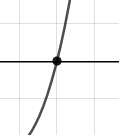
\includegraphics[width = 0.3\textwidth]{../Figures/polyZeroBehaviorCopyDA.png}
\end{multicols}\item None of the above.\end{enumerate}
\textbf{General Comment:} You will need to sketch the entire graph, then zoom in on the zero the question asks about.
}
\litem{
Which of the following equations \textit{could} be of the graph presented below?

\begin{center}
    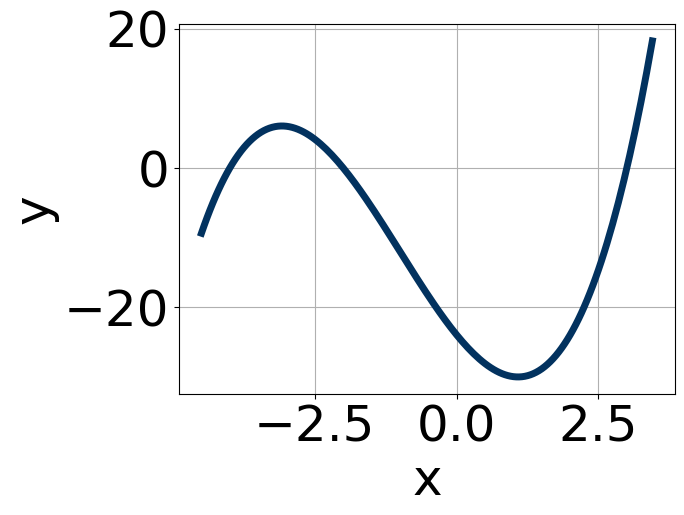
\includegraphics[width=0.5\textwidth]{../Figures/polyGraphToFunctionCopyA.png}
\end{center}


The solution is \( 12x^{4} (x - 3)^{11} (x + 2)^{11} \), which is option C.\begin{enumerate}[label=\Alph*.]
\item \( -10x^{8} (x - 3)^{5} (x + 2)^{7} \)

This corresponds to the leading coefficient being the opposite value than it should be.
\item \( -5x^{8} (x - 3)^{9} (x + 2)^{4} \)

The factor $(x + 2)$ should have an odd power and the leading coefficient should be the opposite sign.
\item \( 12x^{4} (x - 3)^{11} (x + 2)^{11} \)

* This is the correct option.
\item \( 11x^{4} (x - 3)^{10} (x + 2)^{7} \)

The factor $(x - 3)$ should have an odd power.
\item \( 19x^{7} (x - 3)^{8} (x + 2)^{9} \)

The factor $0$ should have an even power and the factor $3$ should have an odd power.
\end{enumerate}

\textbf{General Comment:} General Comments: Draw the x-axis to determine which zeros are touching (and so have even multiplicity) or cross (and have odd multiplicity).
}
\litem{
Describe the end behavior of the polynomial below.
\[ f(x) = -5(x - 9)^{3}(x + 9)^{6}(x - 7)^{3}(x + 7)^{5} \]The solution is the graph below, which is option A.
\begin{center}
    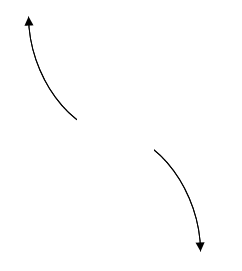
\includegraphics[width=0.3\textwidth]{../Figures/polyEndBehaviorCopyAA.png}
\end{center}\begin{enumerate}[label=\Alph*.]
\begin{multicols}{2}
\item 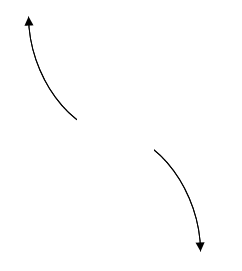
\includegraphics[width = 0.3\textwidth]{../Figures/polyEndBehaviorCopyAA.png}
\item 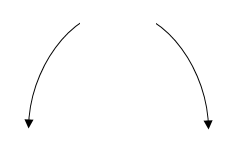
\includegraphics[width = 0.3\textwidth]{../Figures/polyEndBehaviorCopyBA.png}
\item 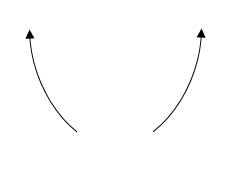
\includegraphics[width = 0.3\textwidth]{../Figures/polyEndBehaviorCopyCA.png}
\item 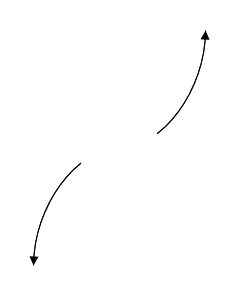
\includegraphics[width = 0.3\textwidth]{../Figures/polyEndBehaviorCopyDA.png}
\end{multicols}\item None of the above.\end{enumerate}
\textbf{General Comment:} Remember that end behavior is determined by the leading coefficient AND whether the \textbf{sum} of the multiplicities is positive or negative.
}
\litem{
Construct the lowest-degree polynomial given the zeros below. Then, choose the intervals that contain the coefficients of the polynomial in the form $x^3+bx^2+cx+d$.
\[ -4 + 2 i \text{ and } -3 \]The solution is \( x^{3} +11 x^{2} +44 x + 60 \), which is option C.\begin{enumerate}[label=\Alph*.]
\item \( b \in [-17, -4], c \in [38, 48], \text{ and } d \in [-61, -58] \)

$x^{3} -11 x^{2} +44 x -60$, which corresponds to multiplying out $(x-(-4 + 2 i))(x-(-4 - 2 i))(x -3)$.
\item \( b \in [-4, 7], c \in [6, 11], \text{ and } d \in [7, 18] \)

$x^{3} + x^{2} +7 x + 12$, which corresponds to multiplying out $(x + 4)(x + 3)$.
\item \( b \in [6, 12], c \in [38, 48], \text{ and } d \in [59, 70] \)

* $x^{3} +11 x^{2} +44 x + 60$, which is the correct option.
\item \( b \in [-4, 7], c \in [-3, 2], \text{ and } d \in [-8, -3] \)

$x^{3} + x^{2} +x -6$, which corresponds to multiplying out $(x -2)(x + 3)$.
\item \( \text{None of the above.} \)

This corresponds to making an unanticipated error or not understanding how to use nonreal complex numbers to create the lowest-degree polynomial. If you chose this and are not sure what you did wrong, please contact the coordinator for help.
\end{enumerate}

\textbf{General Comment:} Remember that the conjugate of $a+bi$ is $a-bi$. Since these zeros always come in pairs, we need to multiply out $(x-(-4 + 2 i))(x-(-4 - 2 i))(x-(-3))$.
}
\litem{
Describe the end behavior of the polynomial below.
\[ f(x) = -2(x - 2)^{2}(x + 2)^{7}(x + 8)^{3}(x - 8)^{5} \]The solution is the graph below, which is option A.
\begin{center}
    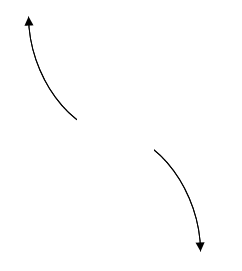
\includegraphics[width=0.3\textwidth]{../Figures/polyEndBehaviorAA.png}
\end{center}\begin{enumerate}[label=\Alph*.]
\begin{multicols}{2}
\item 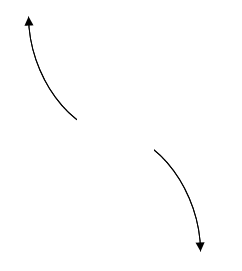
\includegraphics[width = 0.3\textwidth]{../Figures/polyEndBehaviorAA.png}
\item 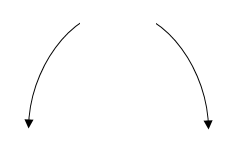
\includegraphics[width = 0.3\textwidth]{../Figures/polyEndBehaviorBA.png}
\item 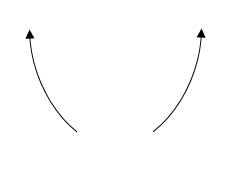
\includegraphics[width = 0.3\textwidth]{../Figures/polyEndBehaviorCA.png}
\item 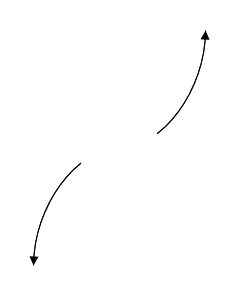
\includegraphics[width = 0.3\textwidth]{../Figures/polyEndBehaviorDA.png}
\end{multicols}\item None of the above.\end{enumerate}
\textbf{General Comment:} Remember that end behavior is determined by the leading coefficient AND whether the \textbf{sum} of the multiplicities is positive or negative.
}
\litem{
Construct the lowest-degree polynomial given the zeros below. Then, choose the intervals that contain the coefficients of the polynomial in the form $x^3+bx^2+cx+d$.
\[ -2 - 4 i \text{ and } -2 \]The solution is \( x^{3} +6 x^{2} +28 x + 40 \), which is option C.\begin{enumerate}[label=\Alph*.]
\item \( b \in [-11, -3], c \in [27.08, 28.99], \text{ and } d \in [-40.7, -36.4] \)

$x^{3} -6 x^{2} +28 x -40$, which corresponds to multiplying out $(x-(-2 - 4 i))(x-(-2 + 4 i))(x -2)$.
\item \( b \in [-3, 5], c \in [4.37, 7.77], \text{ and } d \in [5.9, 8.6] \)

$x^{3} + x^{2} +6 x + 8$, which corresponds to multiplying out $(x + 4)(x + 2)$.
\item \( b \in [2, 15], c \in [27.08, 28.99], \text{ and } d \in [36.9, 41.9] \)

* $x^{3} +6 x^{2} +28 x + 40$, which is the correct option.
\item \( b \in [-3, 5], c \in [2.08, 5.16], \text{ and } d \in [2.9, 4.7] \)

$x^{3} + x^{2} +4 x + 4$, which corresponds to multiplying out $(x + 2)(x + 2)$.
\item \( \text{None of the above.} \)

This corresponds to making an unanticipated error or not understanding how to use nonreal complex numbers to create the lowest-degree polynomial. If you chose this and are not sure what you did wrong, please contact the coordinator for help.
\end{enumerate}

\textbf{General Comment:} Remember that the conjugate of $a+bi$ is $a-bi$. Since these zeros always come in pairs, we need to multiply out $(x-(-2 - 4 i))(x-(-2 + 4 i))(x-(-2))$.
}
\litem{
Construct the lowest-degree polynomial given the zeros below. Then, choose the intervals that contain the coefficients of the polynomial in the form $ax^3+bx^2+cx+d$.
\[ 5, \frac{-7}{4}, \text{ and } \frac{-4}{5} \]The solution is \( 20x^{3} -49 x^{2} -227 x -140 \), which is option E.\begin{enumerate}[label=\Alph*.]
\item \( a \in [19, 30], b \in [-50, -45], c \in [-227, -224], \text{ and } d \in [140, 146] \)

$20x^{3} -49 x^{2} -227 x + 140$, which corresponds to multiplying everything correctly except the constant term.
\item \( a \in [19, 30], b \in [46, 52], c \in [-227, -224], \text{ and } d \in [140, 146] \)

$20x^{3} +49 x^{2} -227 x + 140$, which corresponds to multiplying out $(x + 5)(4x -7)(5x -4)$.
\item \( a \in [19, 30], b \in [142, 154], c \in [277, 289], \text{ and } d \in [140, 146] \)

$20x^{3} +151 x^{2} +283 x + 140$, which corresponds to multiplying out $(x + 5)(4x + 7)(5x + 4)$.
\item \( a \in [19, 30], b \in [77, 83], c \in [-125, -118], \text{ and } d \in [-140, -135] \)

$20x^{3} +81 x^{2} -123 x -140$, which corresponds to multiplying out $(x + 5)(4x -7)(5x + 4)$.
\item \( a \in [19, 30], b \in [-50, -45], c \in [-227, -224], \text{ and } d \in [-140, -135] \)

* $20x^{3} -49 x^{2} -227 x -140$, which is the correct option.
\end{enumerate}

\textbf{General Comment:} To construct the lowest-degree polynomial, you want to multiply out $(x -5)(4x + 7)(5x + 4)$
}
\end{enumerate}

\end{document}